\documentclass[11pt, a4paper]{article}

\usepackage{amsmath}
\usepackage{amsfonts} %Matheschriften
\usepackage{amssymb} %Mathesymbole
%\usepackage{mathptmx} % Einstellung für Schriften und Sonderzeichen in mathematischen Umgebungen
                        % ändert SChriftfont
\usepackage{wasysym} % Stellt diverse Sonderzeichen bereit
\usepackage{siunitx}
\usepackage{float}
\usepackage{microtype}
\usepackage{graphicx}
\usepackage{hyperref}
\usepackage{xcolor}
\usepackage[section]{placeins}


\usepackage[ngerman]{babel}
\addto\captionsngerman{%
 \renewcommand{\abstractname}{Einleitung}}

\title{Versuch 4: Pohlsches Rad}
\author{Jascha Fricker, Benedict Brouwer}

\begin{document}
    \maketitle

    

    \begin{abstract}
        In diesen Versuch wird ein gedämpfter harmonischer Oszillator untersucht. Harmonische Oszillatoren
        sind ein wichtiges Modell in der Physik, da sie sehr viele systeme in der realen Welt beschreiben können.
        Ein berühmtes Thema sind z. B. Resonanzkatastrophen, bei dehnen große Bauwerke in iherer Eingenschwingung
        angeregt werden. Genau solche Schwingungen eines getriebenen Harmonischen Oszillators werden auch in diesem
        Versuch untersucht.
    \end{abstract}

    \tableofcontents

    \newpage

    \section{Stromabhängigkeit der Dämpfungskonstanten}
    \subsection{Theorie}
    Je nachdem wie stark ein harmonischer Oszillator gedämpft wird, ändert sich seine Schwingfrequenz.
    Ein gedämpfter harmonischer Oszillator hat die Bewegungsgleichung
    \begin{align}
        \varphi(t) = \varphi_0 \cdot exp(-\lambda t) \cdot cos(\omega_d - \beta), \label{theo5}
    \end{align}
    mit Kreisfrequenz $\omega_d = \sqrt{\frac{k}{\Theta} - \lambda^2}$ (Drehmoment $\Theta$ und Federkonstante $k$)
    und $\beta$ als Phasenverschiebung. Diese kann aus der Differentialgleichung der Kräfte 
    hergeleitet werden (siehe Aufgabenblatt \cite[(5)]{POR}).
    Bei der in diesem Experiment benutzten Wirbelstrombremse ist die
    Dämpfungskonstante $\lambda$ proportional zum Quadrat des Stroms $I$ durch die Bremse.
    \begin{align}
        \lambda \propto I^2.
    \end{align}

    \subsection{Experimenteller Aufbau}
    Die Stromstärke der Wirbelstrombremse wurde mit einem Labornetzteil eingestellt und
    mit einem VC130 Multimeter gemessen. Nachdem das Pohlsche Rad fast maximal ausgelenkt worden war, 
    wurde der Winkel des Pohlschen Rades abhängig von der Zeit
    mit einem Hall Sensor gemessen und direkt digital aufgenommen.

    \subsection{Auswertung}
    Um die Eingenfrequenz und Dämpfungskonsante abhängig von der Stromstärke zu bestimmen,
    wurde auf jede Messreihe einzeln mit
    der Funkion \textsf{optimize.curve\_fit} der Pythonbibliothek scipy die Theoriekurve \ref{theo5}
    gefittet und auch die Unsicherheit ausgerechnet. Mit diesen 2x15 Datenpunkten können jetzt die Zusammenhänge
    zwischen $\omega_d, \lambda$ und $I$ untersucht werden.

    \subsection{Ergebnis}
    \begin{figure}
        \centering
        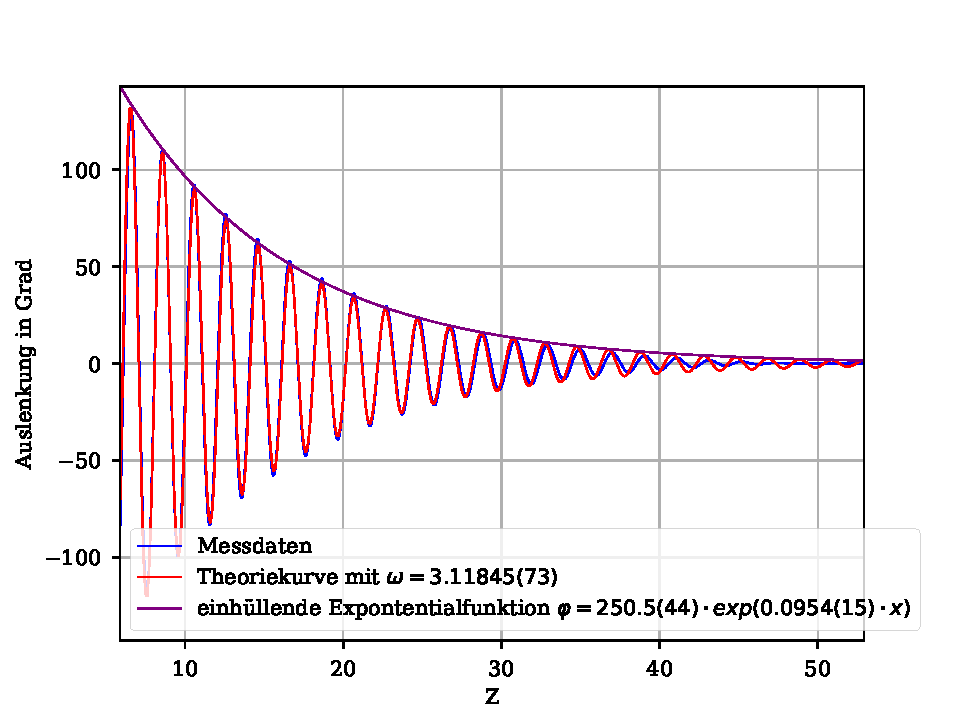
\includegraphics[width=\textwidth]{./8comp.pdf}

        \caption{Messung der Eigenfrequenz}
        \label{fig:eigenfrequenz}
    \end{figure}


    \section{Schwingungsverhalten bei gegebener Dämpfung}
    \subsection{Theorie}

    Bei gegebener Dämpfung hat der Oszillator eine charakteristische Eigenfrequenz.
    Die Eigenfrequenz eines Oszillators lässt sich mithilfe der Schwingungsperiode $T$ berechnen
    \begin{align}
        \omega_d = \frac{2\pi}{T}
    \end{align}

    Bei einer gedämpften Schwingung hat die Bewegungsgleichung
    \begin{align}
        \varphi(t) = \varphi_0 \cdot exp(-\lambda t) \cdot cos(\omega_d - \beta), \label{theo5}
    \end{align}
    deshalb liegen alle Maxima der Ausschläge des Pohlschen Rades auf der einhüllenden Exponentialfunktion
    \begin{align}
        \varphi(t_n) &= \varphi_0 \cdot exp(-\lambda t_n).
    \end{align}
    Die Abklingzeit
    \begin{align}
        \tau = \frac{1}{\lambda}
    \end{align}
    ist der Kehrwert der Dämpfungskonstante.

    Bei einem gezwungenen Oszillator mit Drehmoment $M_0 sin(\omega t)$ kommt noch die partikuläre Lösung zur Bewegungsgleichung
    \begin{align}
        \varphi(t) &= A(\omega) \cdot sin(\omega t - \varphi) + C \cdot exp(-\lambda t) \cdot cos(\omega_d - \beta) \\
        \text{mit Amplitude}  \ \ A(\omega) &= \frac{M_o}{\varphi \sqrt{}}
    \end{align}

    \subsection{Experimenteller Aufbau}
    Für das ganze Experiment wurde ein Dämpfungsstrom von $0,3 \si{\ampere}$ gewählt.
    Um die Eingenfrequenz händisch zu Messen, wurde 5 Mal die Zeit für 10 Schwingungen gemessen.
    Die maximale Amplitude wurde händisch jede SChwingung bestimmt, was sehr schnelles Aufschreiben erfordert.
    Außerdem wurde eine Messreihe digital aufgenommen, um die Eigenfrequenz und Dämpfungskonstante mit dem Computer zu bestimmen.
    Um die REsonanzkurve zu  messen, wurde das Pohlsche Rad mit einem SChrittmotor angetrieben. Die maximale Amplitude wurde
    wurde digital bestimmt.

    \subsection{Auswertung}
    Die von Hand gemessen Periodendauern können direkt ausgewertet werden, an die Computerdaten
    wird wie im ersten Versuch die Theoriekurve gefittet. Auch für die Dämpfungskonstante und für die
    Resonanzkurve wird programmatisch eine Theoriekurve angelegt, um die Ergebnisse mit Unsicherheit
    zu bestimmen. Die Dämpfungskonstante wird aus der einhülleden Exponentialfunktion bestimmt.
n
    \subsection{Ergebnis}
    \subsubsection{Eigenfrequenz und Dämpfungskonstante}
    \begin{figure}
        \centering
        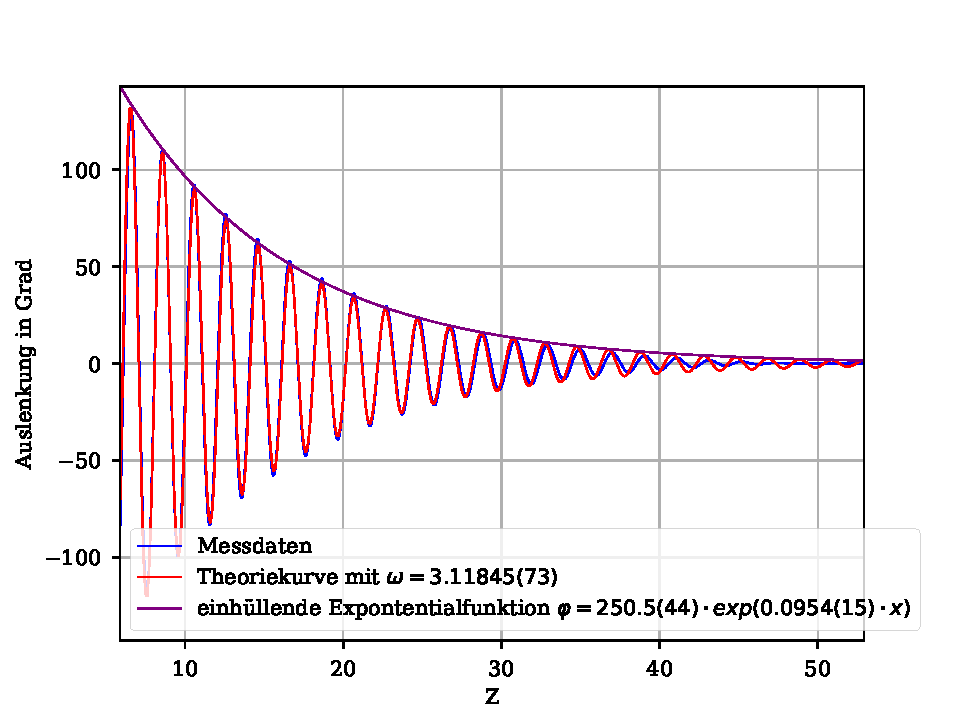
\includegraphics[width=\textwidth]{./8comp.pdf}

        \caption{Messung der Eigenfrequenz}
        \label{fig:eigenfrequenz}
    \end{figure}
    \begin{figure}
        \centering
        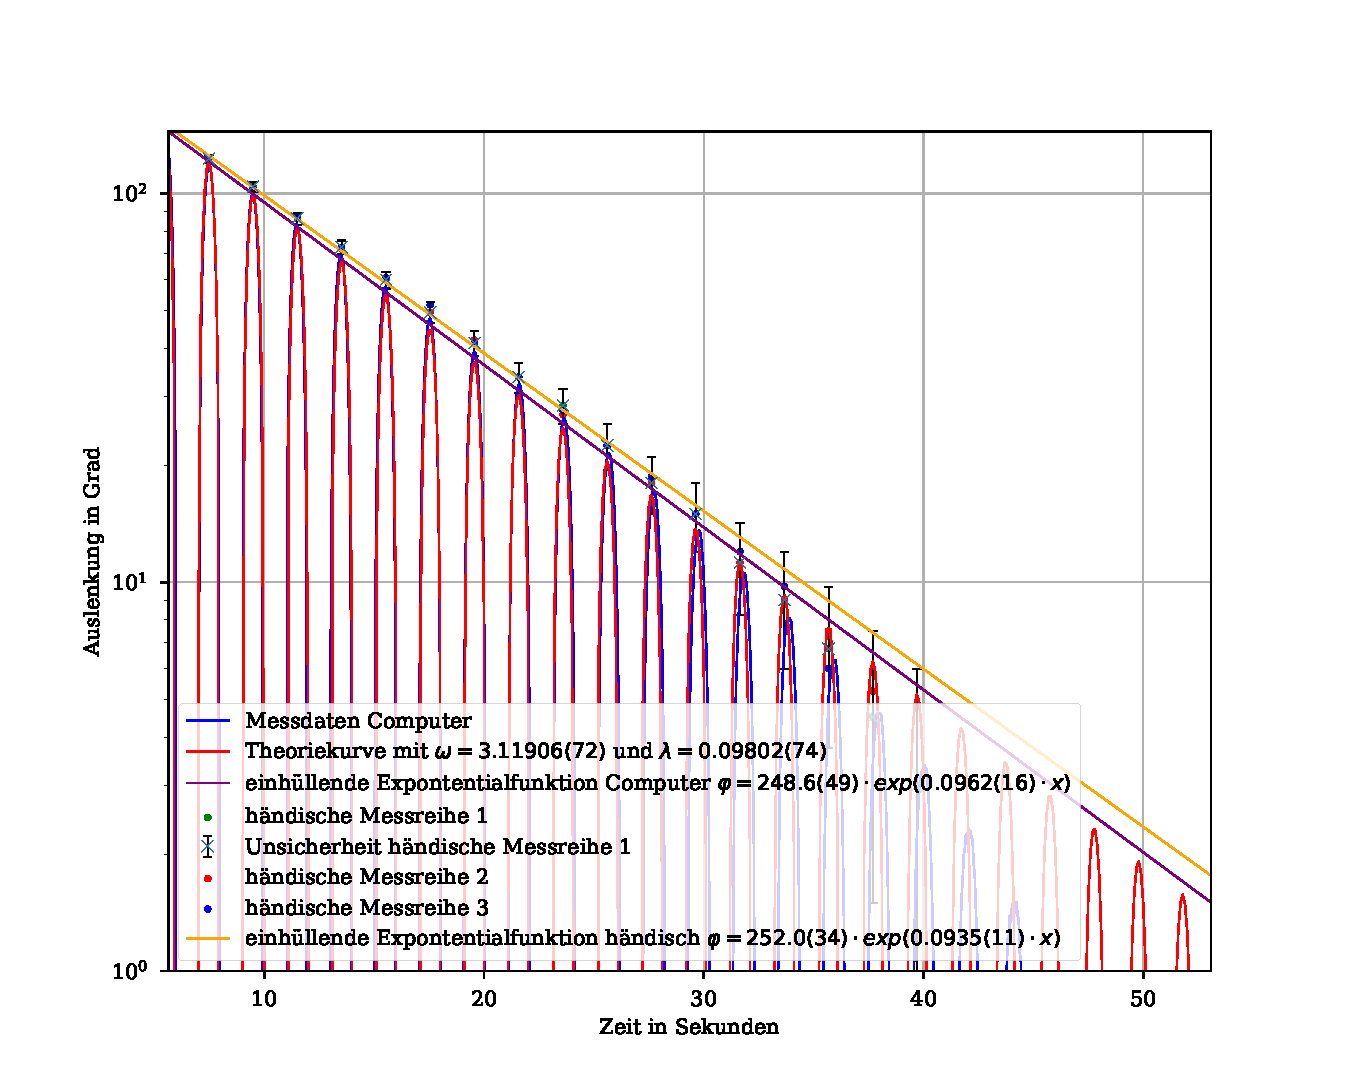
\includegraphics[width=\textwidth]{./9all.pdf}

        \caption{Messung der Dämpfungskonstante}
        \label{fig:daempfung}
    \end{figure}
    In Graph \ref{fig:eigenfrequenz} kann die digitale Messung und die gefittete
    Funktion gesehen werden. Die gleiche einhüllende Exponentialfunktion sowie die Daten der händischen Amplitudenmessung
    wurden im Graphen \ref{fig:daempfung} halblogarithmisch dargestellt.
    
    Als Fehler wurden bei der händischen Messung der Eigenfrequenz berücksichtigt, die Ungenauigkeit der Stuppuhr hingegen
    wurde vernachlässigt, da sie um größenordnungen kleiner ist. Bei der Amplitudenmessung wird eine Unsicherheit von ca 2 Strichen
    oder $3^{\circ}$ angenommen, da die Daten schnell abgelesen werden müssen.
    In Tabelle \ref{Tab:tableeig} wird die händisch gemessene Dämpfungskonstante und Eigenfrequenz (Herleitung siehe Anhang ?) sowie die
    digital gemessene Dämpfungskonstante und Eigenfrequenz angegeben. 
    \begin{table}[H]
        \centering
        \begin{tabular}{c c c} 
            & Hand & Computer \\ \hline
            Eigenfrequenz $\omega$ & $3,118(24) \si{\radian\per\second}$ & $3.11913(74) \si{\radian\per\second}$ \\
            Dämpfungskonstante $\lambda$ & $0,0935(11)$ & $0.0962(16)$

            
        \end{tabular}
        \caption{Eigenfrequenz im Vergleich}
        \label{Tab:tableeig}
    \end{table}

    \bibliographystyle{plain}
    \bibliography{literature}

\end{document}